% !TEX root =../prj4projektrapport.tex

\section{Distributionslinje}

Til simulering af distributionslinjen skulle kabellængde og kabelparametre bestemmes. For kabelparametre blev der i samarbejde med vejleder valgt en kabeltype fra nkt cables, se bilag B1.For kabellængden kontaktede projektgruppen energiselskabet Eniig og modtog et kortudsnit fra deres netbase, se bilag C2. Længden af distributionslinjer i kortudsnittet er relativt korte, og med de valgte kabelparametre, 0,10 $\Omega$/km og 0,22 mH/km, vil dette ikke påvirke spændingen. For at få en påvirkning fra kablet vælges det derfor at simulere en distributionslinje med længde 60 km\footnote{Projektdokumentation, 8.1, Distributionslinje}.  

\subsection{Design og implementering}

På baggrund af de valgte kabelparametre og tilgængelige komponenter, er simuleringen af Distributionslinjen implementeret med værdierne 6,2 $\Omega$ og 13,6 mH gennem to modstande og to spoler i serie. Til den centrale Måleenhed implementeres også en 1 $\Omega$ modstand. Den implementerede distributionslinje ses på figur \ref{fig:DisbLinje}.

\begin{figure}[H]
	\centering
	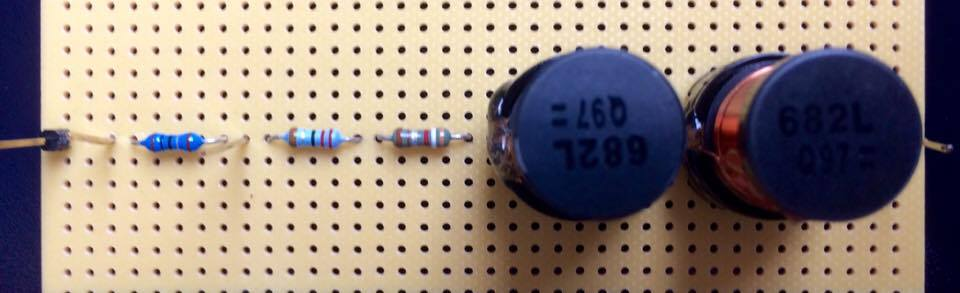
\includegraphics[width=0.7\textwidth]{figure/Distributionslinje}
	\caption{Færdigt print med Distributionslinje}
	\label{fig:DisbLinje}
\end{figure}
